\documentclass[tikz, border=12pt]{standalone}
\usepackage{tikz}
\usetikzlibrary{positioning, arrows.meta, shapes.geometric, fit, backgrounds, calc}

\definecolor{commander}{HTML}{1B2A4A}
\definecolor{agent}{HTML}{3B5BA9}
\definecolor{tool}{HTML}{1C8C7C}
\definecolor{synthetic}{HTML}{6B7280}
\definecolor{live}{HTML}{C7622A}
\definecolor{guard}{HTML}{B38600}
\definecolor{alertbox}{HTML}{4A4A4A}
\definecolor{outbox}{HTML}{214D3E}
\definecolor{edge}{HTML}{3F3F46}
\definecolor{panelbg}{HTML}{F4F5F7}

\begin{document}
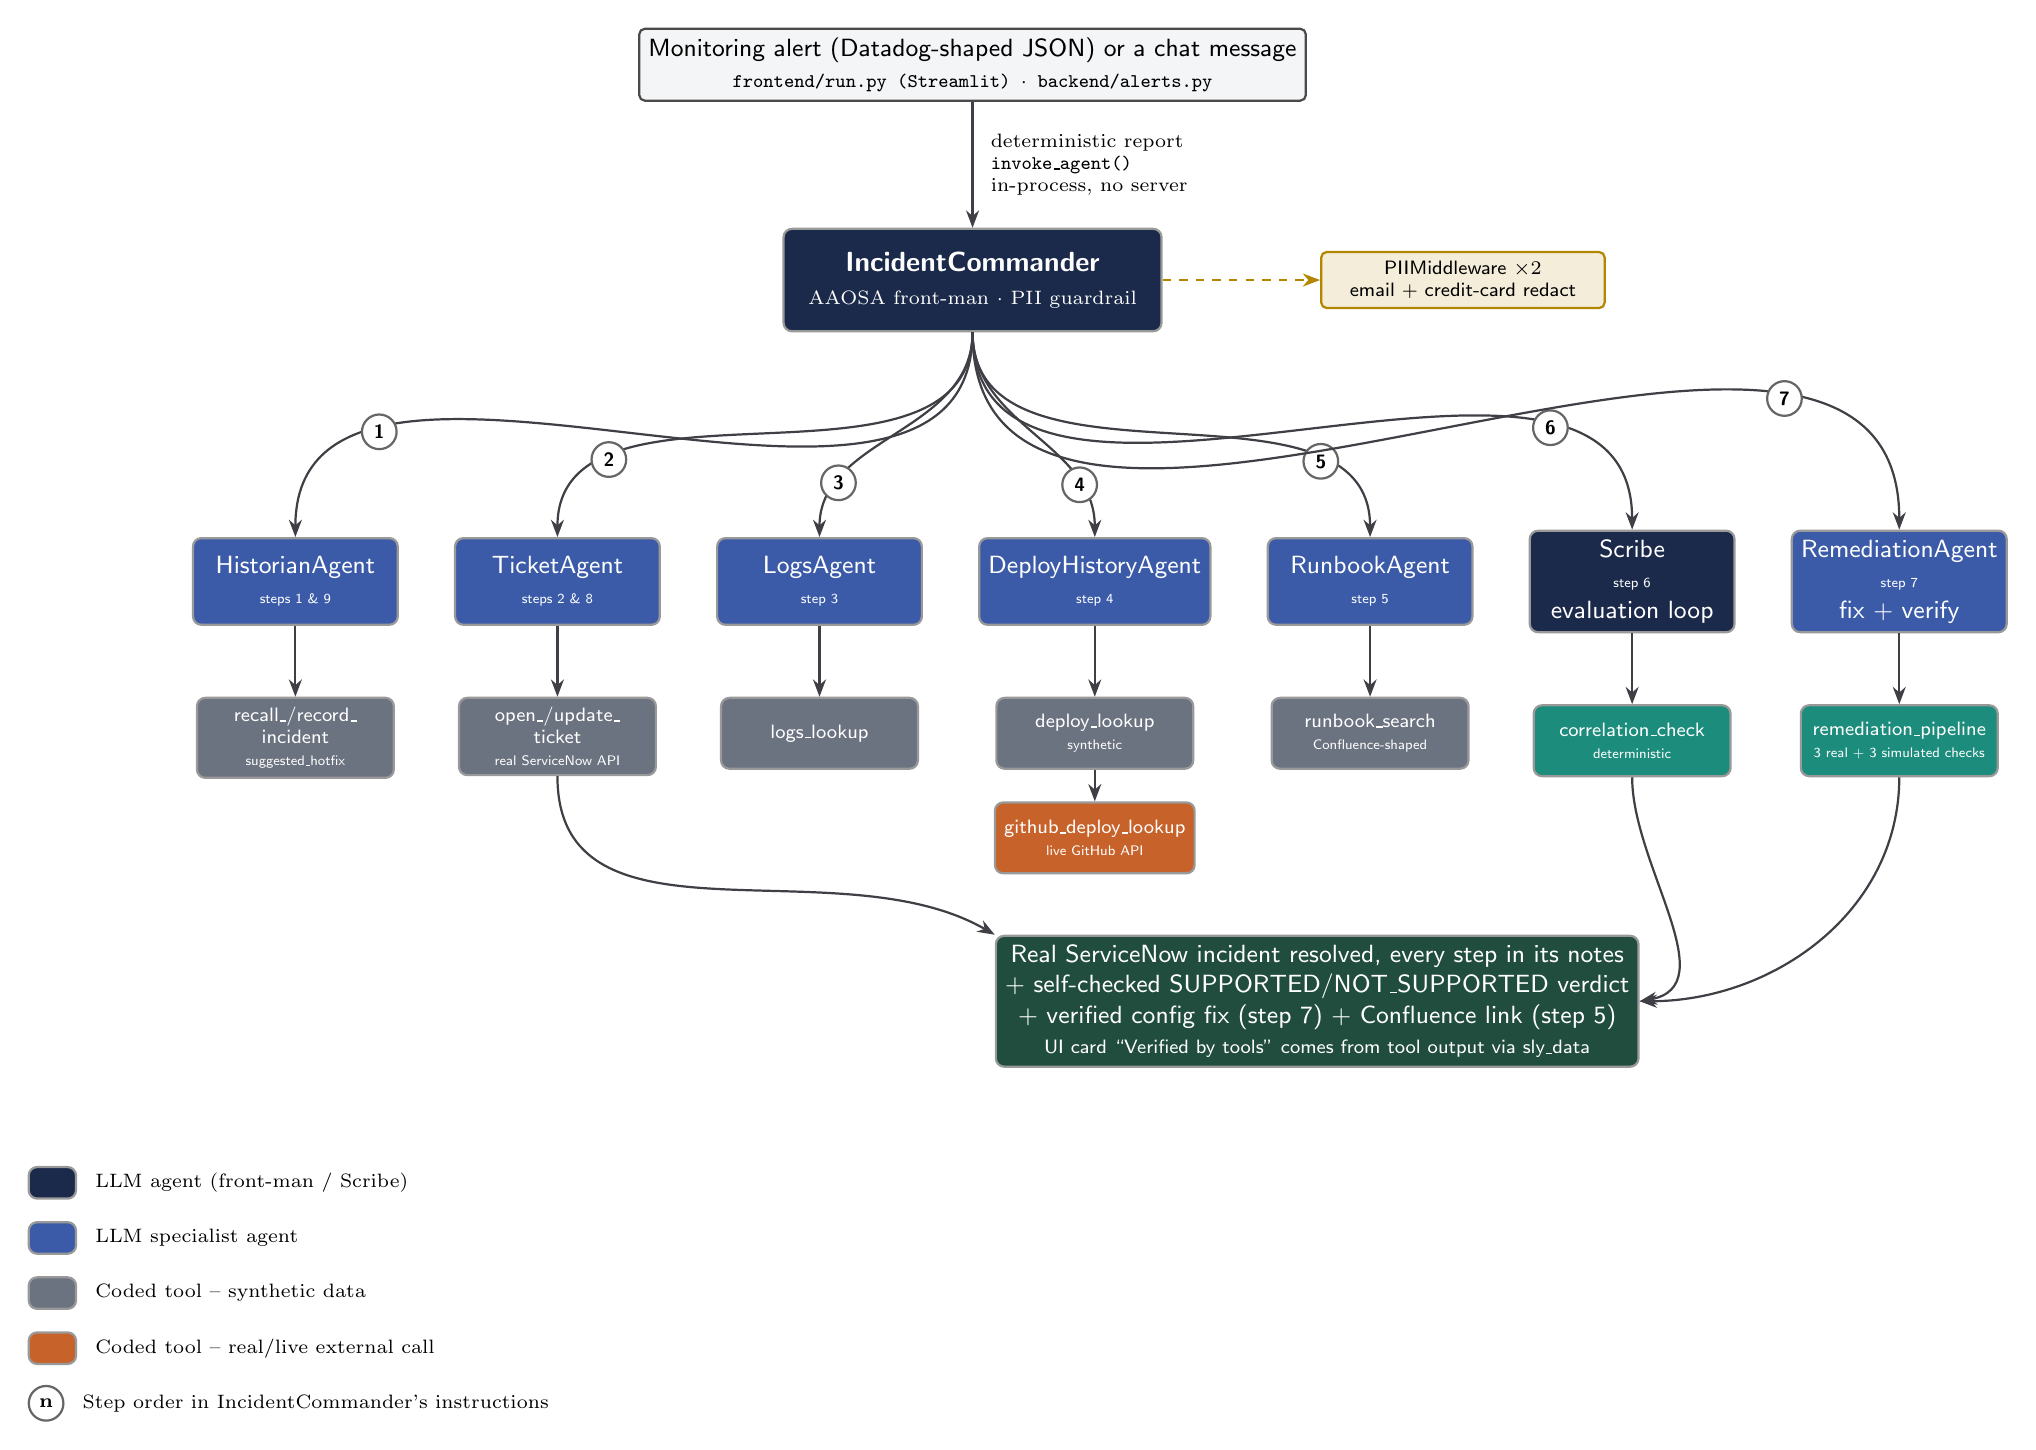
\begin{tikzpicture}[
  font=\sffamily,
  >=Stealth,
  thick,
  node distance=11mm and 7mm,
  every node/.style={align=center},
  box/.style={rounded corners=3pt, draw=black!40, minimum height=9mm, text=white, font=\sffamily\small},
  commanderbox/.style={box, fill=commander, minimum width=48mm, minimum height=13mm, font=\sffamily\bfseries\normalsize},
  agentbox/.style={box, fill=agent, minimum width=26mm, minimum height=11mm, font=\sffamily\small},
  specialbox/.style={box, fill=commander, minimum width=26mm, minimum height=11mm, font=\sffamily\small},
  toolbox/.style={box, fill=tool, minimum width=25mm, minimum height=9mm, font=\sffamily\scriptsize},
  syntool/.style={toolbox, fill=synthetic},
  livetool/.style={toolbox, fill=live},
  ext/.style={rounded corners=2pt, draw=alertbox, fill=panelbg, text=black, minimum width=52mm, minimum height=9mm, font=\sffamily\small},
  outnode/.style={rounded corners=3pt, draw=black!40, fill=outbox, text=white, minimum width=72mm, minimum height=15mm, font=\sffamily\small},
  edg/.style={-{Stealth[length=2.2mm]}, color=edge},
  stepnum/.style={circle, draw=black!60, fill=white, text=black, font=\sffamily\scriptsize\bfseries, inner sep=1pt, minimum size=4.4mm},
]

% ---- External alert source ----
\node[ext, minimum width=74mm] (alert) {Monitoring alert (Datadog-shaped JSON) or a chat message\\\scriptsize \ttfamily frontend/run.py (Streamlit)\ $\cdot$\ backend/alerts.py};

% ---- Commander ----
\node[commanderbox, below=16mm of alert] (cmd) {IncidentCommander\\\scriptsize\normalfont AAOSA front-man\ $\cdot$\ PII guardrail};
\draw[edg] (alert) -- node[right, font=\scriptsize, text=black, align=left, xshift=1mm]{deterministic report\\\ttfamily invoke\_agent()\\\scriptsize in-process, no server} (cmd);

\node[rounded corners=2pt, draw=guard, fill=guard!15, text=black, font=\sffamily\scriptsize, minimum width=36mm, minimum height=7mm, right=20mm of cmd] (guardnote) {PIIMiddleware $\times2$\\email + credit-card redact};
\draw[edg, color=guard, dashed] (cmd) -- (guardnote);

% ---- Row of 6 agents (5 specialists/support + Scribe), evenly spaced ----
\node[agentbox, below=26mm of cmd, xshift=-86mm] (hist) {HistorianAgent\\\tiny steps 1 \& 9};
\node[agentbox, right=of hist] (tick) {TicketAgent\\\tiny steps 2 \& 8};
\node[agentbox, right=of tick] (logs) {LogsAgent\\\tiny step 3};
\node[agentbox, right=of logs] (depl) {DeployHistoryAgent\\\tiny step 4};
\node[agentbox, right=of depl] (rbok) {RunbookAgent\\\tiny step 5};
\node[specialbox, right=of rbok] (scribe) {Scribe\\\tiny step 6 \\ evaluation loop};
\node[agentbox, right=of scribe] (remed) {RemediationAgent\\\tiny step 7 \\ fix + verify};

% ---- Commander -> each agent, single clean edge per box ----
\foreach \n/\lbl in {hist/1, tick/2, logs/3, depl/4, rbok/5, scribe/6, remed/7} {
  \draw[edg] (cmd.south) to[out=-90, in=90] node[stepnum, pos=0.78]{\lbl} (\n.north);
}

% ---- Coded tools beneath each agent ----
\node[syntool, below=9mm of hist] (t_recall) {recall\_/record\_\\incident\\\tiny suggested\_hotfix};
\node[syntool, below=9mm of tick] (t_ticket) {open\_/update\_\\ticket\\\tiny real ServiceNow API};
\node[syntool, below=9mm of logs] (t_logs) {logs\_lookup};
\node[syntool, below=9mm of depl] (t_deploy) {deploy\_lookup\\\tiny synthetic};
\node[livetool, below=4mm of t_deploy] (t_github) {github\_deploy\_lookup\\\tiny live GitHub API};
\node[syntool, below=9mm of rbok] (t_runbook) {runbook\_search\\\tiny Confluence-shaped};
\node[toolbox, below=9mm of scribe] (t_corr) {correlation\_check\\\tiny deterministic};
\node[toolbox, below=9mm of remed] (t_remed) {remediation\_pipeline\\\tiny 3 real + 3 simulated checks};

\draw[edg] (hist) -- (t_recall);
\draw[edg] (tick) -- (t_ticket);
\draw[edg] (logs) -- (t_logs);
\draw[edg] (depl.south) -- (t_deploy.north);
\draw[edg] (t_deploy.south) -- (t_github.north);
\draw[edg] (rbok) -- (t_runbook);
\draw[edg] (scribe) -- (t_corr);
\draw[edg] (remed) -- (t_remed);

% ---- Final output ----
\node[outnode, below=20mm of t_corr, xshift=-40mm] (out) {Real ServiceNow incident resolved, every step in its notes\\
  + self-checked SUPPORTED/NOT\_SUPPORTED verdict\\
  + verified config fix (step 7) + Confluence link (step 5)\\
  \scriptsize UI card ``Verified by tools'' comes from tool output via sly\_data};
\draw[edg] (t_remed.south) to[out=-90, in=0] (out.east);
\draw[edg] (t_corr.south) to[out=-90, in=10] (out.east);
\draw[edg] (t_ticket.south) to[out=-90, in=150] (out.north west);

% ---- Legend ----
\begin{scope}[shift={(-12,-14.2)}]
\node[box, fill=commander, minimum width=6mm, minimum height=4mm, anchor=west] (lg1) at (0,0) {};
\node[right=1mm of lg1, text=black, font=\scriptsize, anchor=west] {LLM agent (front-man / Scribe)};
\node[agentbox, minimum width=6mm, minimum height=4mm, anchor=west] (lg2) at (0,-0.7) {};
\node[right=1mm of lg2, text=black, font=\scriptsize, anchor=west] {LLM specialist agent};
\node[syntool, minimum width=6mm, minimum height=4mm, anchor=west] (lg3) at (0,-1.4) {};
\node[right=1mm of lg3, text=black, font=\scriptsize, anchor=west] {Coded tool -- synthetic data};
\node[livetool, minimum width=6mm, minimum height=4mm, anchor=west] (lg4) at (0,-2.1) {};
\node[right=1mm of lg4, text=black, font=\scriptsize, anchor=west] {Coded tool -- real/live external call};
\node[circle, draw=black!60, fill=white, font=\scriptsize\bfseries, inner sep=1pt, minimum size=4.4mm, anchor=west] (lg5) at (0,-2.8) {n};
\node[right=1mm of lg5, text=black, font=\scriptsize, anchor=west] {Step order in IncidentCommander's instructions};
\end{scope}

\end{tikzpicture}
\end{document}
